
%(BEGIN_QUESTION)
% Copyright 2011, Tony R. Kuphaldt, released under the Creative Commons Attribution License (v 1.0)
% This means you may do almost anything with this work of mine, so long as you give me proper credit

Read and outline Case History \#50 (``Sometimes You Have To Use A Filter'') from Michael Brown's collection of control loop optimization tutorials.  Prepare to thoughtfully discuss with your instructor and classmates the concepts and examples explored in this reading, and answer the following questions:

\begin{itemize}
\item{} Process variable filtering is also known by another term: {\it damping}.  Most transmitters have a programmable damping feature in them, as well as most controller PV inputs, which may be set to provide a wide range of signal filtering.  Explain what this ``filtering'' does to the process variable signal.
\vskip 10pt
\item{} Figure 1 of this report shows the closed-loop trend for a liquid level control system, slowly settling down to setpoint with much oscillation.  It is a fair assessment that the main problem in this loop is a controller that is tuned too aggressively, as opposed to an instrument problem such as friction in the valve.  Explain how we can tell this from the shapes of the PV and Output waves.
\vskip 10pt
\item{} Figure 1 of this report shows the closed-loop trend of PV and Output for a level control system.  Given that the controller is reverse-acting, determine which is the dominant control action (P, I, or D) in this over-tuned controller by examining the {\it phase shift} between PV and Output.
\vskip 10pt
\item{} As far as industrial processes are concerned, the amount of noise present on this PV signal is not extreme.  However, it was a bit too much for the PID tuning recommended by the Protuner software.  Identify how we typically tune (integrating) level control processes, and why this particular tuning does not agree well with a noisy PV signal.
\vskip 10pt
\item{} Explain how Mr. Brown was able to overcome the noise problem in this process, to use the PID tuning parameters suited for this (integrating) process type.
\end{itemize}

\vskip 20pt \vbox{\hrule \hbox{\strut \vrule{} {\bf Suggestions for Socratic discussion} \vrule} \hrule}

\begin{itemize}
\item{} Discuss in general how we may use PV/Output phase shift to identify a controller's dominant action, based on the information contained in the ``Recognizing an Over-Tuned Controller by phase shift'' subsection of the ``Heuristic PID Tuning Procedures'' section of the ``Process Dynamics and PID Controller Tuning'' chapter in your {\it Lessons In Industrial Instrumentation} textbook and discuss this with your classmates.
\item{} Identify the controller's mode (i.e. auto or manual) in each of the trend graphs shown in this article.
\item{} Mr. Brown mentions something at the beginning of this article about an {\it anti-aliasing filter}.  Explain what ``aliasing'' is, and why a low-pass filter helpsto guard against it.  Note that your {\it Lessons In Industrial Instrumentation} textbook discusses this concept.
\end{itemize}

\underbar{file i01790}
%(END_QUESTION)





%(BEGIN_ANSWER)

``Filtering'' or ``damping'' is a low-pass frequency function that is placed either physically or digitally on the process variable signal, in order to screen out high-frequency noise on the PV signal.

%(END_ANSWER)





%(BEGIN_NOTES)

Figure 1's closed-loop test shows both PV and PD waves to be sinusoidal, indicating an over-tuned controller rather than a problem such as valve hysteresis.

\vskip 10pt

Figure 1 reveals a PD (Output) waveform that lags behind the PV waveform in time.  This suggests moderate integral action, which may cause setpoint overshoot and oscillation in integrating processes such as liquid level control.

\vskip 10pt

Level processes typically respond well to aggressive proportional action, but here the noise on the PV would prohibit strong gain (because this would amplify noise to the valve).  

\vskip 10pt

Aggressive gain was made possible by applying some filtering (damping) to the PV signal.





\vfil \eject

\noindent
{\bf Summary Quiz:}

Identify the dominant control action (P, I, or D) in this over-tuned controller, assuming it is {\it direct-acting}:

$$\includegraphics[width=15.5cm]{i01790x01.eps}$$


%INDEX% Reading assignment: Michael Brown Case History #50, "Sometimes you have to use a filter"

%(END_NOTES)


